% Sección de experimentación del Entregable 2 (se incluye desde informe_e2.tex).

\subsection{Metodología}

Los cuatro experimentos están automatizados (\code{python -m benchmarks.run\_all --only 5 6 7 8}) y
guardan CSV y PNG en \code{benchmarks/results/}. Cada uno crea archivos nuevos en una carpeta de
trabajo, con semilla fija. Salvo donde se indica, las consultas se ejecutan \textbf{por SQL sobre el
motor completo} (\code{Database.execute}), de modo que las lecturas incluyen traer los registros de
la tabla, y se toman del \code{DiskCounter} con su desglose por archivo. Entorno:
Python 3.12.13 en macOS-26.3.1-arm64-arm-64bit (10 núcleos), corrida del 2026-11-13 15:49:19%
.

Como en el Entregable~1, los bloques leídos son deterministas y son la métrica principal; los tiempos
dependen de la máquina y de la caché de páginas del sistema operativo (los archivos caben en memoria),
por lo que reflejan sobre todo el costo de CPU. El motor no tiene \emph{buffer pool}: cada lectura
informada es una transferencia real de 4\,KB.

%------------------------------------------------------------------------------------------
\subsection{Experimento 5: escalabilidad espacial y maldición de la dimensionalidad}

\paragraph{Parte A: R-Tree frente al recorrido secuencial en 2D.} Puntos (longitud, latitud) dentro
de Lima Metropolitana (70\,\% agrupados alrededor de 25 centros, 30\,\% uniformes), $N\in\{10^4,
5\cdot10^4, 10^5\}$, en una tabla \code{locales(id, nombre, ubicacion)} de 81 registros por página.
Se promedian 40 consultas por configuración con tres caminos: sin índice, con un R-Tree construido
por inserciones (el índice existe antes del \code{COPY}) y con un R-Tree empaquetado con STR
(\code{CREATE INDEX} después de cargar).

\begin{table}[H]
\centering\scriptsize
\resizebox{\ifdim\width>\textwidth\textwidth\else\width\fi}{!}{\begin{tabular}{@{}llrrrrrrr@{}}
\toprule
 & & \multicolumn{2}{c}{Secuencial (Heap)} & \multicolumn{2}{c}{R-Tree (inserciones)} & \multicolumn{2}{c}{R-Tree (STR)} & \\
\cmidrule(lr){3-4}\cmidrule(lr){5-6}\cmidrule(lr){7-8}
$N$ & consulta & lecturas & ms & lecturas & ms & lecturas & ms & filas \\
\midrule
10\,000 & radio 0.5 km & 124.0 & 13.55 & 14.8 & 0.22 & 14.8 & 0.34 & 10.2 \\
 & radio 1 km & 124.0 & 14.52 & 45.7 & 0.39 & 45.5 & 0.56 & 40.0 \\
 & radio 2 km & 124.0 & 13.54 & 151.8 & 1.14 & 150.8 & 0.95 & 143.2 \\
 & radio 5 km & 124.0 & 13.72 & 601.6 & 3.71 & 600.4 & 3.39 & 585.5 \\
 & $k$-NN, $k=5$ & 124.0 & 18.22 & 9.2 & 0.29 & 9.4 & 0.44 & 5.0 \\
 & $k$-NN, $k=20$ & 124.0 & 18.33 & 25.4 & 0.45 & 25.2 & 0.60 & 20.0 \\
 & $k$-NN, $k=50$ & 124.0 & 18.28 & 56.6 & 0.69 & 56.1 & 0.92 & 50.0 \\
\addlinespace
50\,000 & radio 0.5 km & 618.0 & 68.18 & 63.8 & 0.91 & 63.9 & 0.61 & 55.0 \\
 & radio 1 km & 618.0 & 67.78 & 222.8 & 1.82 & 221.3 & 1.66 & 208.8 \\
 & radio 2 km & 618.0 & 67.92 & 756.2 & 5.07 & 751.9 & 5.41 & 731.7 \\
 & radio 5 km & 618.0 & 71.65 & 2\,750.5 & 16.76 & 2\,736.8 & 16.98 & 2\,691.4 \\
 & $k$-NN, $k=5$ & 618.0 & 105.25 & 10.5 & 0.44 & 11.9 & 0.61 & 5.0 \\
 & $k$-NN, $k=20$ & 618.0 & 97.78 & 27.1 & 0.61 & 27.9 & 0.75 & 20.0 \\
 & $k$-NN, $k=50$ & 618.0 & 98.40 & 59.0 & 0.93 & 59.1 & 1.05 & 50.0 \\
\addlinespace
100\,000 & radio 0.5 km & 1\,235.0 & 138.98 & 104.7 & 1.15 & 102.4 & 0.83 & 92.5 \\
 & radio 1 km & 1\,235.0 & 147.25 & 375.1 & 2.56 & 369.8 & 2.81 & 354.6 \\
 & radio 2 km & 1\,235.0 & 137.20 & 1\,270.5 & 7.89 & 1\,259.8 & 8.47 & 1\,232.1 \\
 & radio 5 km & 1\,235.0 & 138.74 & 4\,568.9 & 34.00 & 4\,541.9 & 27.25 & 4\,474.6 \\
 & $k$-NN, $k=5$ & 1\,235.0 & 187.19 & 12.2 & 0.58 & 12.0 & 0.58 & 5.0 \\
 & $k$-NN, $k=20$ & 1\,235.0 & 185.63 & 28.8 & 0.72 & 28.1 & 0.77 & 20.0 \\
 & $k$-NN, $k=50$ & 1\,235.0 & 192.36 & 60.8 & 1.45 & 59.3 & 2.14 & 50.0 \\
\bottomrule
\end{tabular}
}
\caption{Experimento 5A: bloques leídos (índice + tabla) y tiempo por consulta.}
\label{tab:exp5}
\end{table}

\begin{table}[H]
\centering\small
\resizebox{\ifdim\width>\textwidth\textwidth\else\width\fi}{!}{\begin{tabular}{@{}rrrrrrrr@{}}
\toprule
$N$ & páginas del Heap & \multicolumn{3}{c}{R-Tree por inserciones} & \multicolumn{3}{c}{R-Tree STR} \\
\cmidrule(lr){3-5}\cmidrule(l){6-8}
 & & páginas & altura & construcción (s) / escrituras & páginas & altura & construcción (s) / escrituras \\
\midrule
10\,000 & 124 & 141 & 3 & 0.88 / 10\,678 & 96 & 2 & 0.02 / 100 \\
50\,000 & 618 & 696 & 3 & 5.51 / 53\,564 & 475 & 3 & 0.11 / 479 \\
100\,000 & 1\,235 & 1\,402 & 3 & 10.95 / 106\,617 & 946 & 3 & 0.21 / 950 \\
\bottomrule
\end{tabular}
}
\caption{Tamaño y costo de construcción del R-Tree. Para el árbol por inserciones se descuenta el
costo de cargar el Heap.}
\label{tab:exp5build}
\end{table}

\begin{figure}[H]
\centering
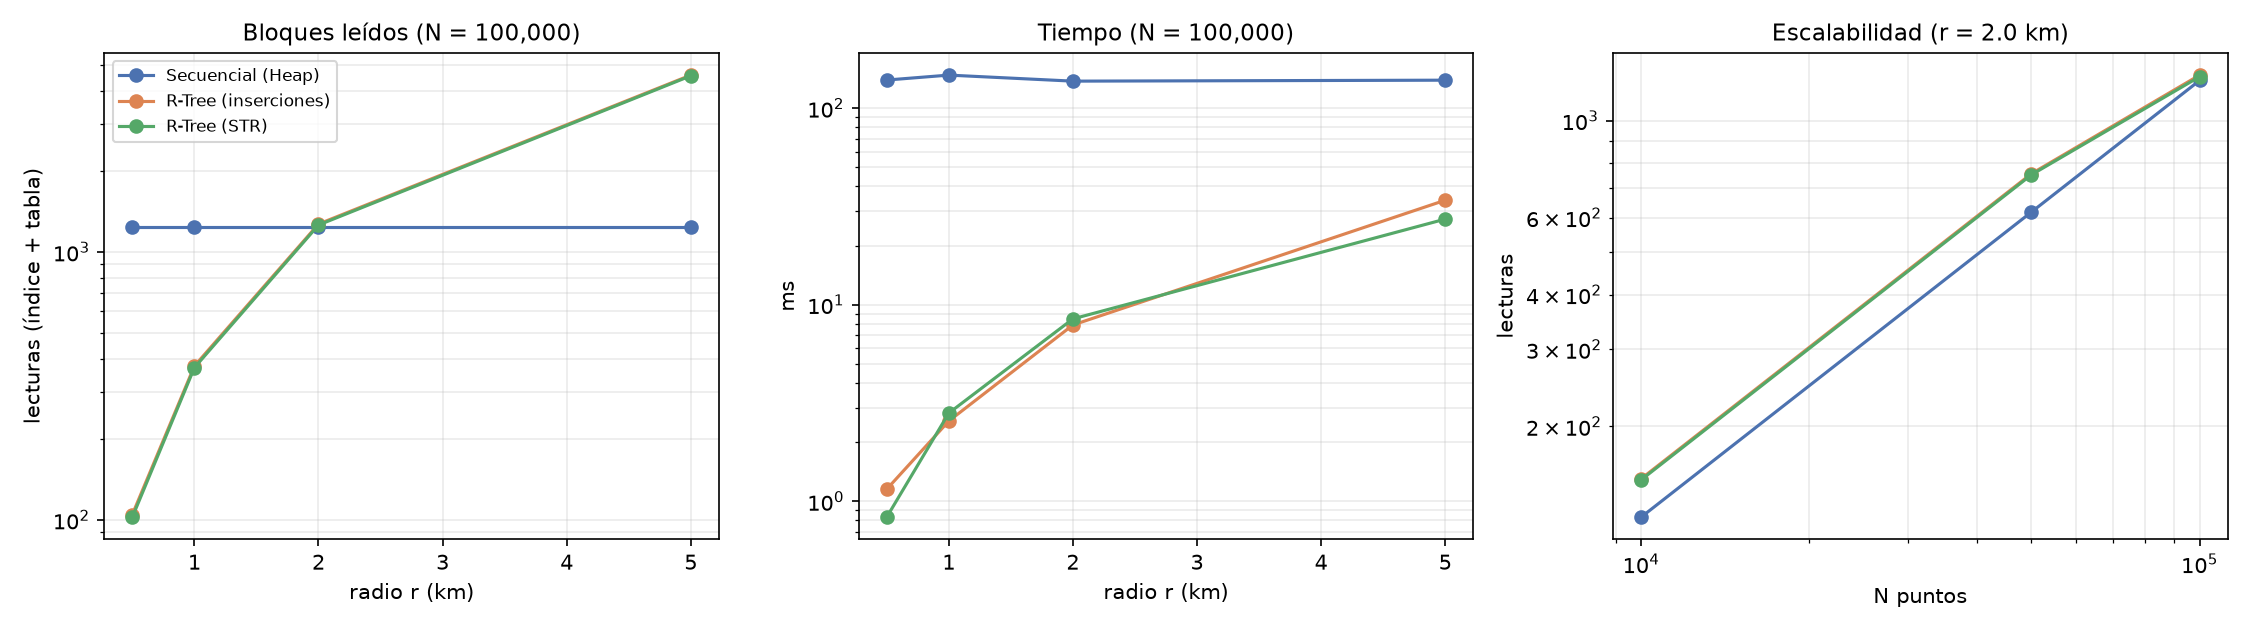
\includegraphics[width=\textwidth]{exp5_radius.png}
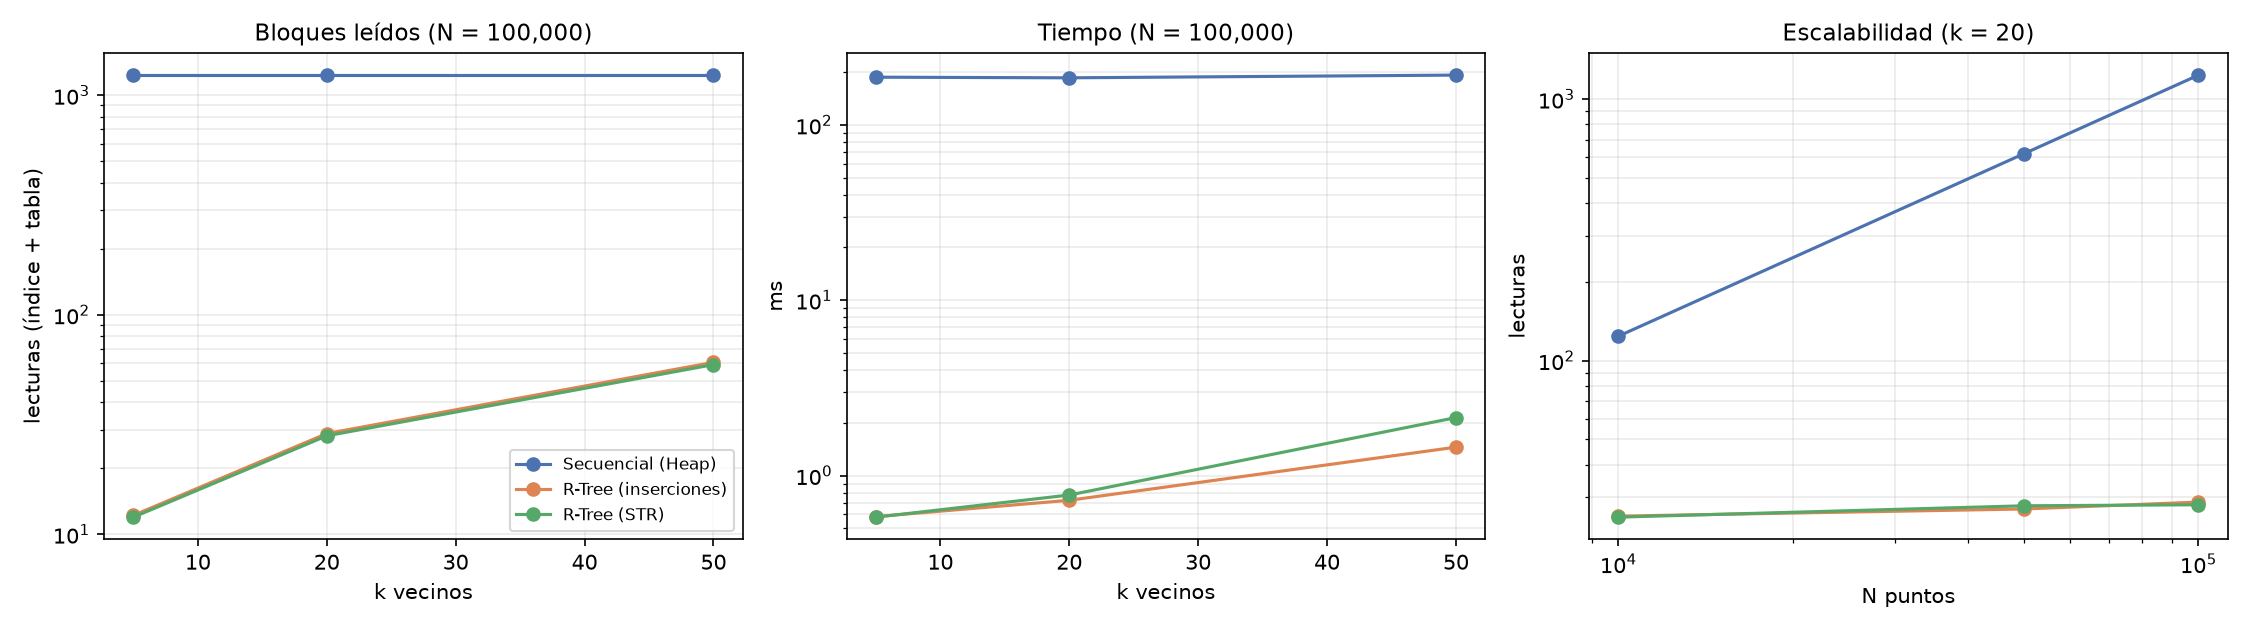
\includegraphics[width=\textwidth]{exp5_knn.png}
\caption{Experimento 5A: consultas por radio (arriba) y $k$-NN (abajo).}
\label{fig:exp5}
\end{figure}

\paragraph{Análisis.}
\begin{itemize}
\item \textbf{$k$-NN}: el R-Tree lee $h$ + unas pocas hojas + $k$ registros. Con $N=10^5$ y $k=5$
  son 12 bloques (7 del índice y 5 de la tabla) frente a los 1\,235 del recorrido secuencial, y el
  costo casi no crece con $N$ (9, 11 y 12 lecturas para $10^4$, $5\cdot10^4$ y $10^5$): solo depende
  de la altura. El recorrido secuencial crece linealmente con $N$.
\item \textbf{Radio}: el índice visita pocos nodos (10 a 94) pero, como no está agrupado, paga una
  lectura de la tabla por cada punto que califica. Con radios pequeños gana por un orden de magnitud
  (102 frente a 1\,235 bloques con $r=0.5$\,km); cuando califican más filas que páginas tiene la
  tabla ($r\ge2$\,km con $N=10^5$) lee \emph{más} bloques que el recorrido secuencial, el mismo
  cruce que observamos con el B$^+$ no agrupado en el Experimento~3. En tiempo sigue ganando (8\,ms
  frente a 137\,ms con $r=2$\,km) porque el recorrido secuencial decodifica y evalúa las $10^5$ filas.
\item \textbf{Inserciones frente a STR}: el árbol empaquetado ocupa un 33\,\% menos de páginas (hojas
  llenas en lugar de $\approx$70\,\%) y se construye con una escritura por página: 950 escrituras
  frente a 106\,617 (cada inserción cuesta $h$ lecturas y al menos una escritura). En consultas ambos
  leen prácticamente lo mismo; el STR visita algo menos de nodos en los radios grandes (67 frente a 94
  con $r=5$\,km) porque sus cajas se solapan menos.
\end{itemize}

\paragraph{Parte B: efecto de la dimensión.} $N=20\,000$ vectores uniformes en $[0,1]^D$ con
coordenadas \code{float32}; $k$-NN con $k=10$ (30 consultas) sobre un R-Tree construido por
inserciones, frente al recorrido secuencial de un Heap con los mismos vectores (ambos con $B=4096$).

\begin{table}[H]
\centering\small
\begin{tabular}{@{}lrrrrrrr@{}}
\toprule
Dimensión $D$ & 2 & 4 & 8 & 16 & 32 & 64 & 128 \\
\midrule
entradas por hoja & 185 & 107 & 58 & 30 & 15 & 7 & 3 \\
altura del R-Tree & 2 & 3 & 3 & 4 & 4 & 6 & 11 \\
páginas del R-Tree & 159 & 279 & 508 & 955 & 1\,745 & 3\,797 & 11\,092 \\
páginas del Heap ($P$) & 60 & 100 & 179 & 339 & 667 & 1\,334 & 2\,858 \\
R-Tree: lecturas por $k$-NN & 12.7 & 21.5 & 100.3 & 952.5 & 1\,754.0 & 3\,806.0 & 11\,100.9 \\
R-Tree: \% de hojas visitadas & 1.1 & 3.2 & 16.4 & 98.7 & 100.0 & 100.0 & 100.0 \\
Secuencial: lecturas & 60 & 100 & 179 & 339 & 667 & 1\,334 & 2\,858 \\
R-Tree: ms por consulta & 0.32 & 1.12 & 4.70 & 42.72 & 51.17 & 79.92 & 190.49 \\
Secuencial: ms por consulta & 7.72 & 11.78 & 9.37 & 13.76 & 12.14 & 18.33 & 31.38 \\
\bottomrule
\end{tabular}

\caption{Experimento 5B: $k$-NN ($k=10$) según la dimensión.}
\label{tab:exp5dim}
\end{table}

\begin{figure}[H]
\centering
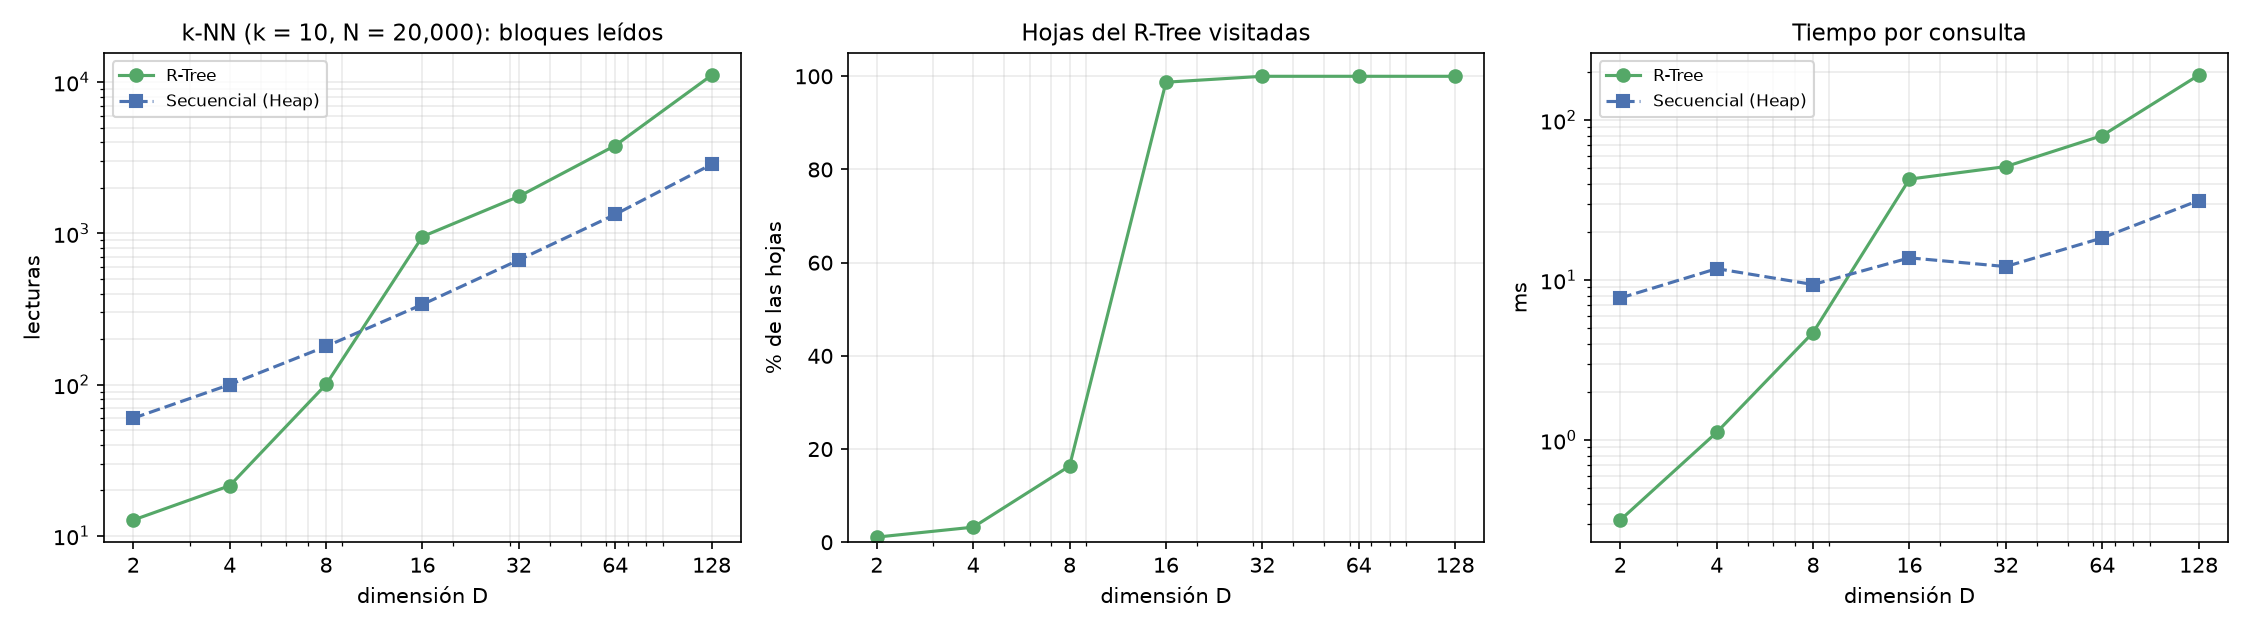
\includegraphics[width=\textwidth]{exp5_dimension.png}
\caption{Experimento 5B: bloques leídos, fracción de hojas visitadas y tiempo según $D$.}
\label{fig:exp5dim}
\end{figure}

\paragraph{Análisis.} El R-Tree gana con claridad en $D=2$ y $D=4$ (13 y 21 lecturas frente a 60 y
100) y todavía en $D=8$ (100 frente a 179), pero \textbf{desde $D=16$ pierde}: visita el 99\,\% de
las hojas y lee 953 bloques frente a los 339 del recorrido secuencial. Actúan dos efectos a la vez.
Primero, la entrada crece como $2Dc$ y el \emph{fan-out} cae de 185 a 3 entradas por página, así que
el árbol tiene más páginas que la propia tabla (11\,092 frente a 2\,858 con $D=128$) y su altura
pasa de 2 a 11. Segundo, en alta dimensión las distancias se concentran: la distancia al vecino más
cercano se parece a la del más lejano, las cajas se solapan y $\text{MINDIST}$ deja de podar, por lo
que el recorrido \emph{best-first} termina abriendo todos los nodos. Es la maldición de la
dimensionalidad: para los vectores de 128 dimensiones de la aplicación un índice espacial exacto no
sirve, y por eso el módulo vectorial usa un índice aproximado (Experimento~8).

%------------------------------------------------------------------------------------------
\subsection{Experimento 6: índice invertido frente a \emph{full scan} y GIN de PostgreSQL}

Corpus: las descripciones de los productos (en inglés, 12.7 términos por documento tras el
preprocesamiento), de 1\,000 a 44\,072 documentos en una tabla \code{docs(id, cuerpo TEXT(200))} de
19 registros por página. PostgreSQL~18 con \code{GIN (to\_tsvector('english', cuerpo))}.

\begin{table}[H]
\centering\small
\resizebox{\ifdim\width>\textwidth\textwidth\else\width\fi}{!}{\begin{tabular}{@{}rrrrrrrrrr@{}}
\toprule
 & \multicolumn{7}{c}{MiniDB: índice invertido en disco} & \multicolumn{2}{c}{PostgreSQL GIN} \\
\cmidrule(lr){2-8}\cmidrule(l){9-10}
documentos & términos & posteos & vocab. & posteos & docs & total (KB) & s & KB & s \\
\midrule
1\,000 & 1\,010 & 12\,722 & 15 & 19 & 4 & 164 & 0.03 & 104 & 0.03 \\
2\,000 & 1\,492 & 25\,377 & 21 & 38 & 8 & 280 & 0.06 & 160 & 0.04 \\
5\,000 & 2\,398 & 63\,538 & 34 & 94 & 20 & 604 & 0.12 & 296 & 0.10 \\
10\,000 & 3\,676 & 127\,061 & 52 & 188 & 40 & 1\,132 & 0.21 & 544 & 0.18 \\
20\,000 & 5\,455 & 254\,178 & 76 & 375 & 80 & 2\,136 & 0.39 & 968 & 0.36 \\
44\,072 & 7\,939 & 560\,112 & 111 & 827 & 174 & 4\,460 & 0.92 & 1\,824 & 0.73 \\
\bottomrule
\end{tabular}
}
\caption{Experimento 6: construcción del índice. Para MiniDB se indican las páginas de cada archivo
(\code{vocab.dic}, \code{postings.inv}, \code{docs.bin}), el tamaño total y el tiempo.}
\label{tab:exp6build}
\end{table}

\begin{figure}[H]
\centering
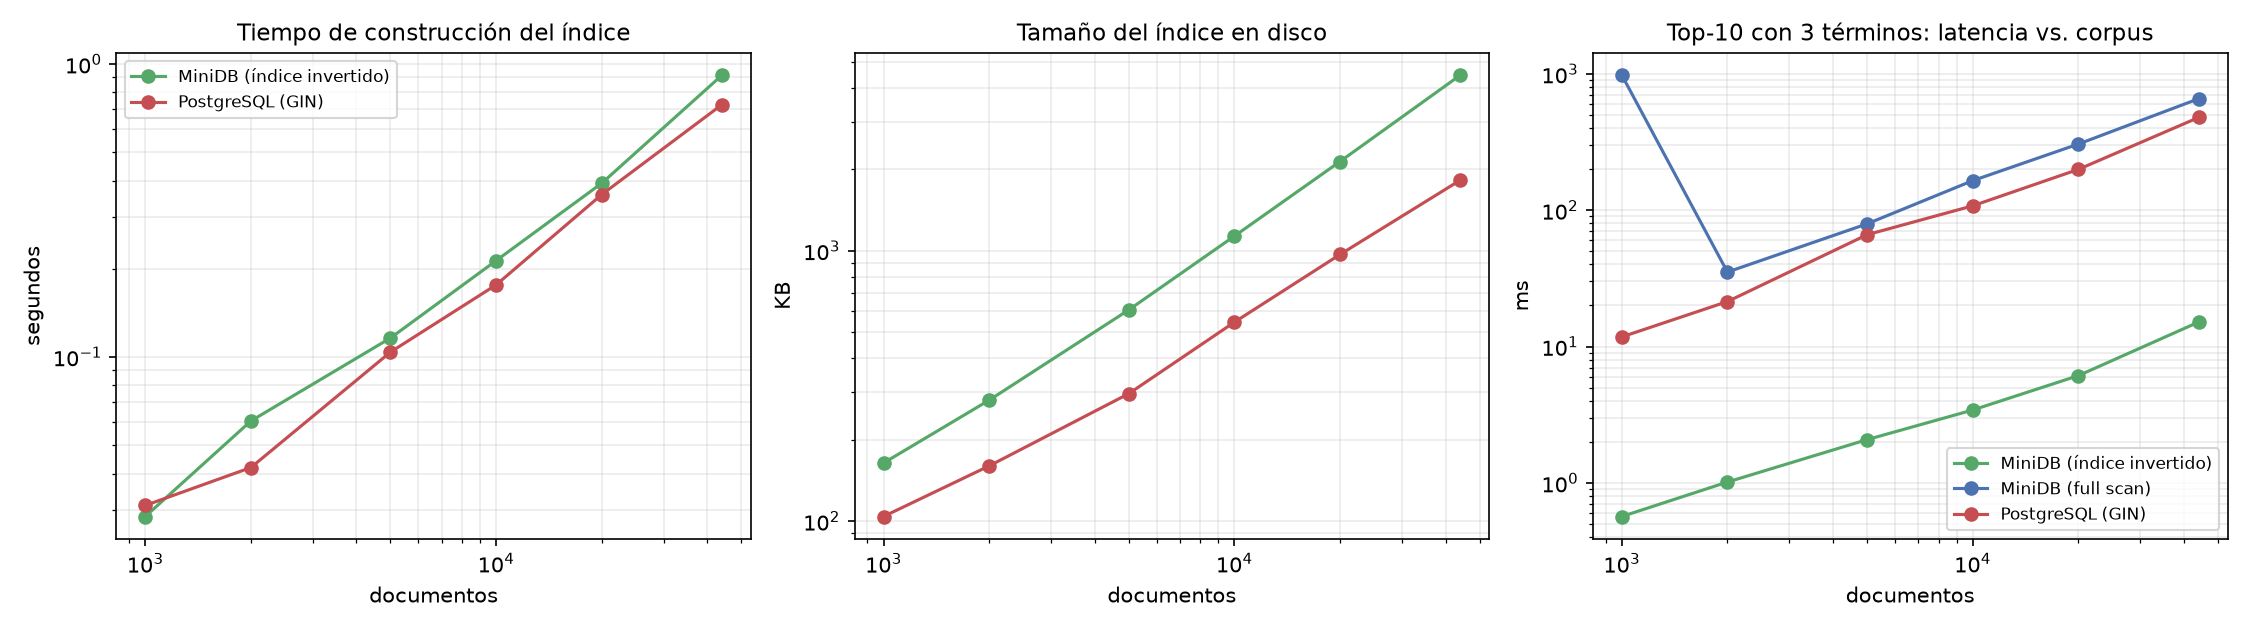
\includegraphics[width=\textwidth]{exp6_build.png}
\caption{Experimento 6: tiempo de construcción, tamaño en disco y latencia del Top-10 de 3 términos
según el tamaño del corpus.}
\label{fig:exp6build}
\end{figure}

\paragraph{Construcción.} El tiempo y el tamaño crecen linealmente con el corpus: el vocabulario
crece de forma sublineal (ley de Heaps: 1\,010 términos con 1\,000 documentos y 7\,939 con 44\,072)
y los posteos de forma lineal (12.7 por documento, 6 bytes cada uno). El índice completo de 44\,072
documentos ocupa 4.5\,MB y se construye en 0.9\,s con 3\,166 lecturas (el recorrido de la tabla y la
relectura del \emph{run}) y 1\,966 escrituras. El GIN de PostgreSQL es 2.4 veces más compacto porque
comprime las listas de posteo y no guarda frecuencias ni normas (por eso su ranking debe recalcular
el \code{tsvector} de cada documento); su tiempo de construcción es similar.

Con el corpus completo se ejecutan 30 consultas por configuración, con términos tomados de un mismo
documento para que tengan resultados (3 consultas en el caso del \emph{full scan}).

\begin{table}[H]
\centering\scriptsize
\resizebox{\ifdim\width>\textwidth\textwidth\else\width\fi}{!}{\begin{tabular}{@{}lrrrrrrrr@{}}
\toprule
 & & \multicolumn{2}{c}{MiniDB (índice invertido)} & \multicolumn{2}{c}{MiniDB (full scan)} & \multicolumn{2}{c}{PostgreSQL (GIN)} & \\
\cmidrule(lr){3-4}\cmidrule(lr){5-6}\cmidrule(lr){7-8}
consulta & términos & ms & bloques & ms & bloques & ms & bloques & filas \\
\midrule
AND & 1 & 70.20 & 13\,577.4 & 608.17 & 2\,320.0 & 2.02 & 681.9 & 13\,470.8 \\
 & 3 & 11.21 & 1\,072.8 & 589.85 & 2\,320.0 & 0.58 & 250.4 & 939.5 \\
 & 5 & 8.62 & 393.8 & 594.63 & 2\,320.0 & 0.52 & 142.7 & 213.9 \\
\addlinespace
OR & 1 & 55.07 & 10\,284.4 & 557.42 & 2\,320.0 & 1.55 & 610.6 & 10\,183.2 \\
 & 3 & 163.23 & 31\,055.6 & 609.24 & 2\,320.0 & 5.12 & 826.1 & 30\,885.4 \\
 & 5 & 215.37 & 39\,937.5 & 614.83 & 2\,320.0 & 7.99 & 837.3 & 39\,703.4 \\
\addlinespace
AND NOT & 1 & 58.15 & 10\,802.3 & 589.86 & 2\,320.0 & 2.30 & 561.1 & 10\,672.6 \\
 & 3 & 11.11 & 1\,246.8 & 594.24 & 2\,320.0 & 0.83 & 282.0 & 1\,084.8 \\
 & 5 & 11.69 & 873.4 & 602.59 & 2\,320.0 & 0.98 & 260.4 & 645.8 \\
\addlinespace
Top-10 & 1 & 5.58 & 128.1 & 625.34 & 2\,320.0 & 201.23 & 678.2 & 10.0 \\
 & 3 & 15.12 & 200.7 & 656.90 & 2\,320.0 & 478.80 & 821.8 & 10.0 \\
 & 5 & 20.76 & 251.8 & 690.45 & 2\,320.0 & 591.06 & 838.5 & 10.0 \\
\bottomrule
\end{tabular}
}
\caption{Experimento 6: latencia y bloques leídos por consulta ($N=44\,072$). MiniDB usa bloques de
4\,KB sin caché; PostgreSQL, \emph{buffers} de 8\,KB. La última columna son las filas que califican
(10 en el Top-10).}
\label{tab:exp6}
\end{table}

\begin{table}[H]
\centering\small
\begin{tabular}{@{}lrrrr@{}}
\toprule
consulta & términos & lecturas en el índice & lecturas en la tabla & filas \\
\midrule
AND & 1 & 106.6 & 13\,470.8 & 13\,470.8 \\
 & 3 & 133.3 & 939.5 & 939.5 \\
 & 5 & 179.9 & 213.9 & 213.9 \\
OR & 1 & 101.2 & 10\,183.2 & 10\,183.2 \\
 & 3 & 170.2 & 30\,885.4 & 30\,885.4 \\
 & 5 & 234.1 & 39\,703.4 & 39\,703.4 \\
AND NOT & 1 & 129.7 & 10\,672.6 & 10\,672.6 \\
 & 3 & 162.0 & 1\,084.8 & 1\,084.8 \\
 & 5 & 227.6 & 645.8 & 645.8 \\
Top-10 & 1 & 118.1 & 10.0 & 10.0 \\
 & 3 & 190.7 & 10.0 & 10.0 \\
 & 5 & 241.8 & 10.0 & 10.0 \\
\bottomrule
\end{tabular}

\caption{Desglose de las lecturas del índice invertido de MiniDB: en el índice (diccionario, posteos
y normas) y en la tabla (un registro por fila devuelta).}
\label{tab:exp6io}
\end{table}

\begin{figure}[H]
\centering
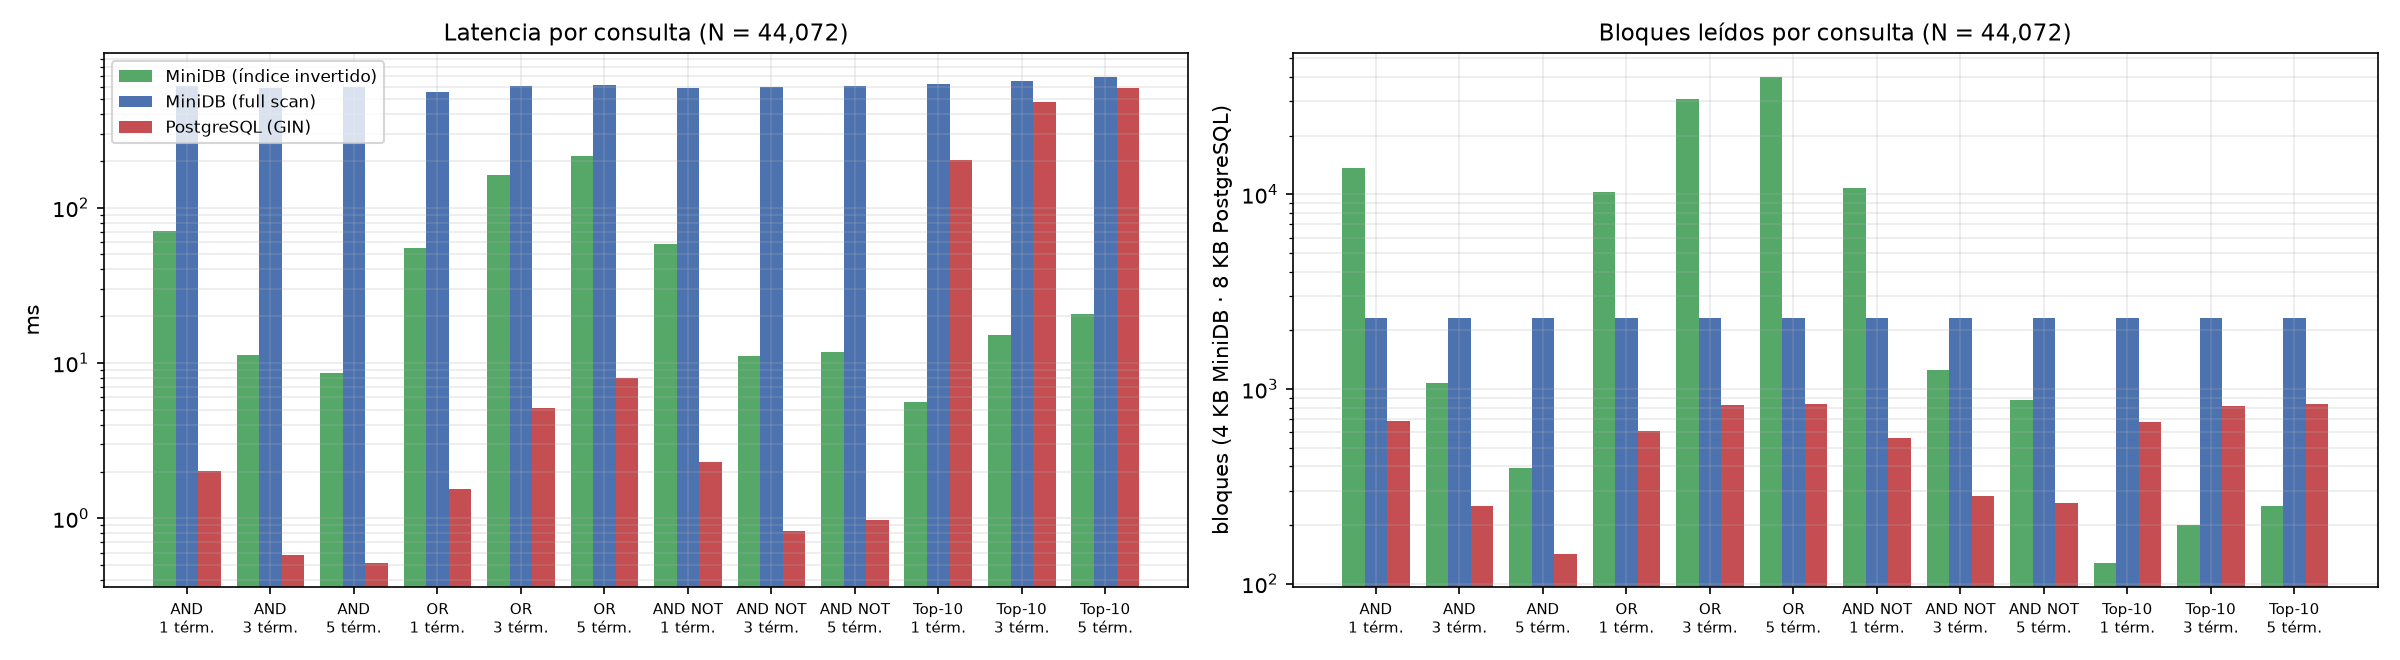
\includegraphics[width=\textwidth]{exp6_queries.png}
\caption{Experimento 6: latencia y bloques leídos por tipo de consulta y número de términos.}
\label{fig:exp6}
\end{figure}

\paragraph{Análisis.}
\begin{itemize}
\item \textbf{Correctitud}: las consultas booleanas devuelven las mismas filas en MiniDB y en
  PostgreSQL (13\,470.8 frente a 13\,469.7 en promedio para un término; las diferencias mínimas
  vienen de las listas de \emph{stopwords}), lo que valida el preprocesamiento y las mezclas con dos
  punteros.
\item \textbf{Índice frente a \emph{full scan}}: el recorrido secuencial lee siempre las 2\,320
  páginas y tokeniza los 44\,072 documentos ($\approx$600\,ms). El índice lee entre 101 y 234 bloques
  propios: $T\lceil\log_2 111\rceil$ del diccionario más las páginas de posteo de cada término. Para
  el Top-10 el total es de 128 a 252 bloques (9 a 18 veces menos que el \emph{full scan}) y la
  latencia de 6 a 21\,ms (30 a 110 veces menos).
\item \textbf{El costo está en traer las filas}: en las consultas booleanas poco selectivas
  (un término, u \code{OR} de varios) califican decenas de miles de documentos y, como el índice
  devuelve RID de un Heap no agrupado, se paga una lectura por fila: 39\,703 lecturas para un
  \code{OR} de 5 términos, más que las 2\,320 del \emph{full scan}. Es el mismo cruce de los índices
  no agrupados. Con \code{AND} de 3 o 5 términos (cientos de filas) el índice vuelve a ganar, y el
  ranking Top-$K$ evita el problema porque solo trae $K$ registros.
\item \textbf{Frente a GIN}: en consultas booleanas PostgreSQL es de 15 a 35 veces más rápido (está
  escrito en C, usa \emph{buffer pool} y un \emph{bitmap heap scan} que lee cada página de la tabla
  una sola vez, con $\approx$50 filas por página de 8\,KB). En el \textbf{ranking Top-10 MiniDB es de
  28 a 36 veces más rápido} (5.6 a 20.8\,ms frente a 201 a 591\,ms): GIN no guarda frecuencias ni
  normas, así que \code{ts\_rank} tiene que recalcular el \code{tsvector} de \emph{todos} los
  documentos que califican antes de ordenar, mientras que nuestro índice tiene $tf$ en los posteos y
  la norma precalculada en \code{docs.bin}, y solo trae de la tabla los 10 ganadores.
\item \textbf{Escalabilidad} (figura~\ref{fig:exp6build}, derecha): la latencia del Top-10 crece
  linealmente con el corpus en los tres sistemas, pero con pendientes muy distintas, porque el índice
  solo recorre las listas de los términos de la consulta.
\end{itemize}

%------------------------------------------------------------------------------------------
\subsection{Experimento 7: BoVW frente a \emph{embeddings} densos}

300 imágenes de consulta: 20 de cada uno de los 15 tipos de artículo más frecuentes. Para cada una
se recuperan sus 10 vecinos (excluida la propia imagen) por SQL sobre la tabla \code{productos}; un
resultado es relevante si es del mismo tipo de artículo.

\begin{table}[H]
\centering\small
\resizebox{\ifdim\width>\textwidth\textwidth\else\width\fi}{!}{\begin{tabular}{@{}lrrrrrrr@{}}
\toprule
Representación & P@5 & P@10 & extracción (ms/imagen) & consulta (ms) & lecturas & en el índice & índice (MB) \\
\midrule
BoVW (SIFT + índice invertido) & 0.531 & 0.505 & 7.70 & 133.68 & 646.0 & 635.0 & 17.0 \\
Embedding (ResNet-18 + IVF) & 0.811 & 0.789 & 7.80 & 6.11 & 215.6 & 204.6 & 25.1 \\
Embedding (k-NN exacto) & 0.811 & 0.786 & 7.80 & 850.25 & 22\,036.0 & 0.0 & -- \\
\bottomrule
\end{tabular}
}
\caption{Experimento 7: precisión, tiempo de extracción por imagen (medido una a una, como en una
consulta de la aplicación) y costo de la consulta.}
\label{tab:exp7}
\end{table}

\begin{figure}[H]
\centering
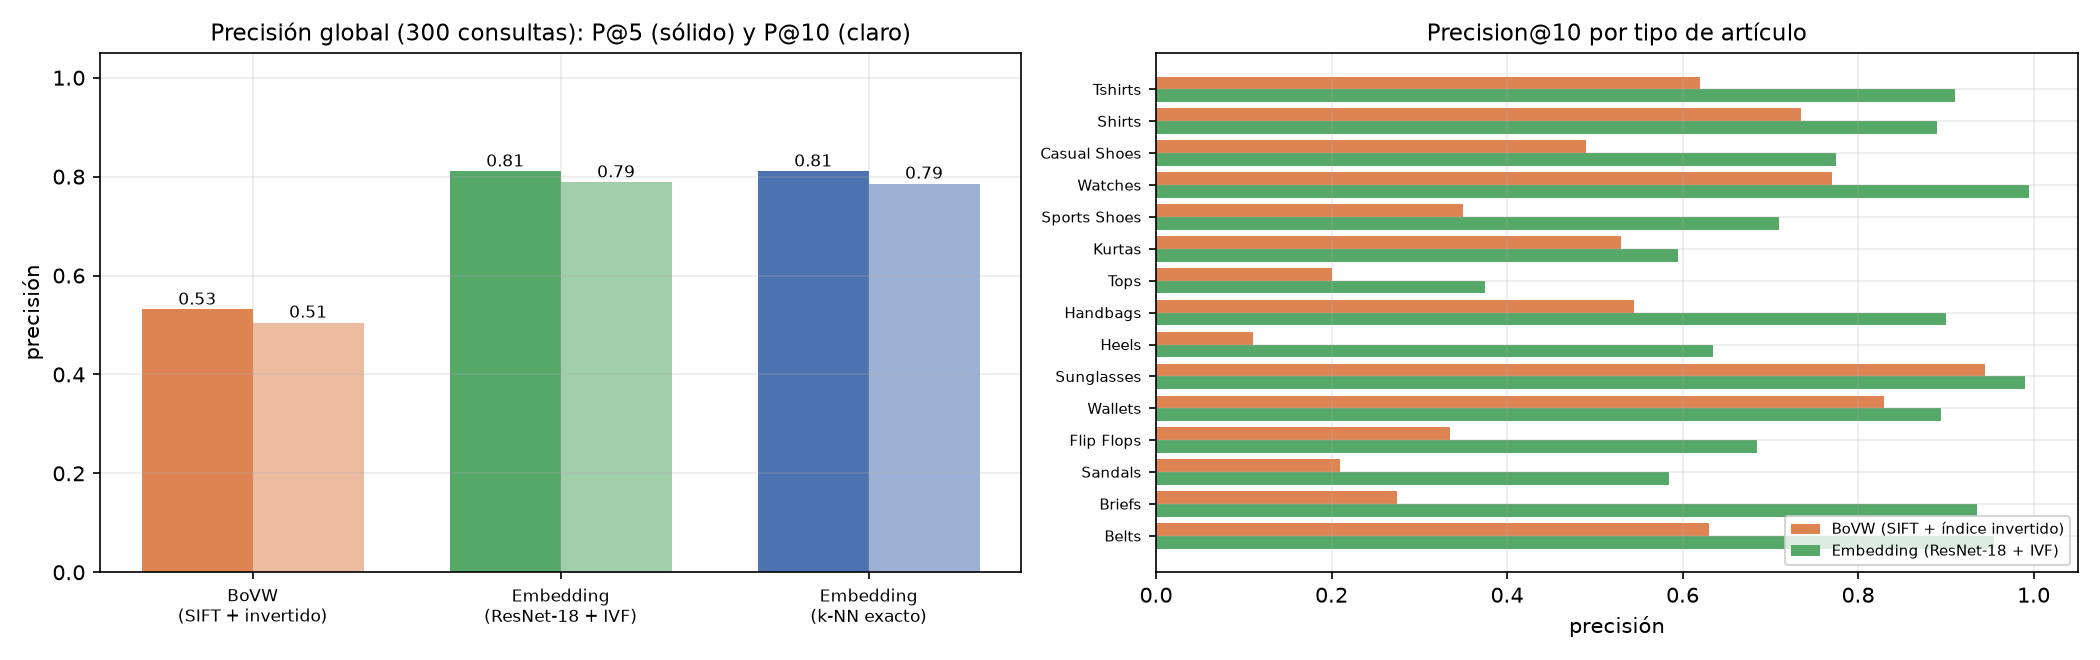
\includegraphics[width=\textwidth]{exp7_precision.png}
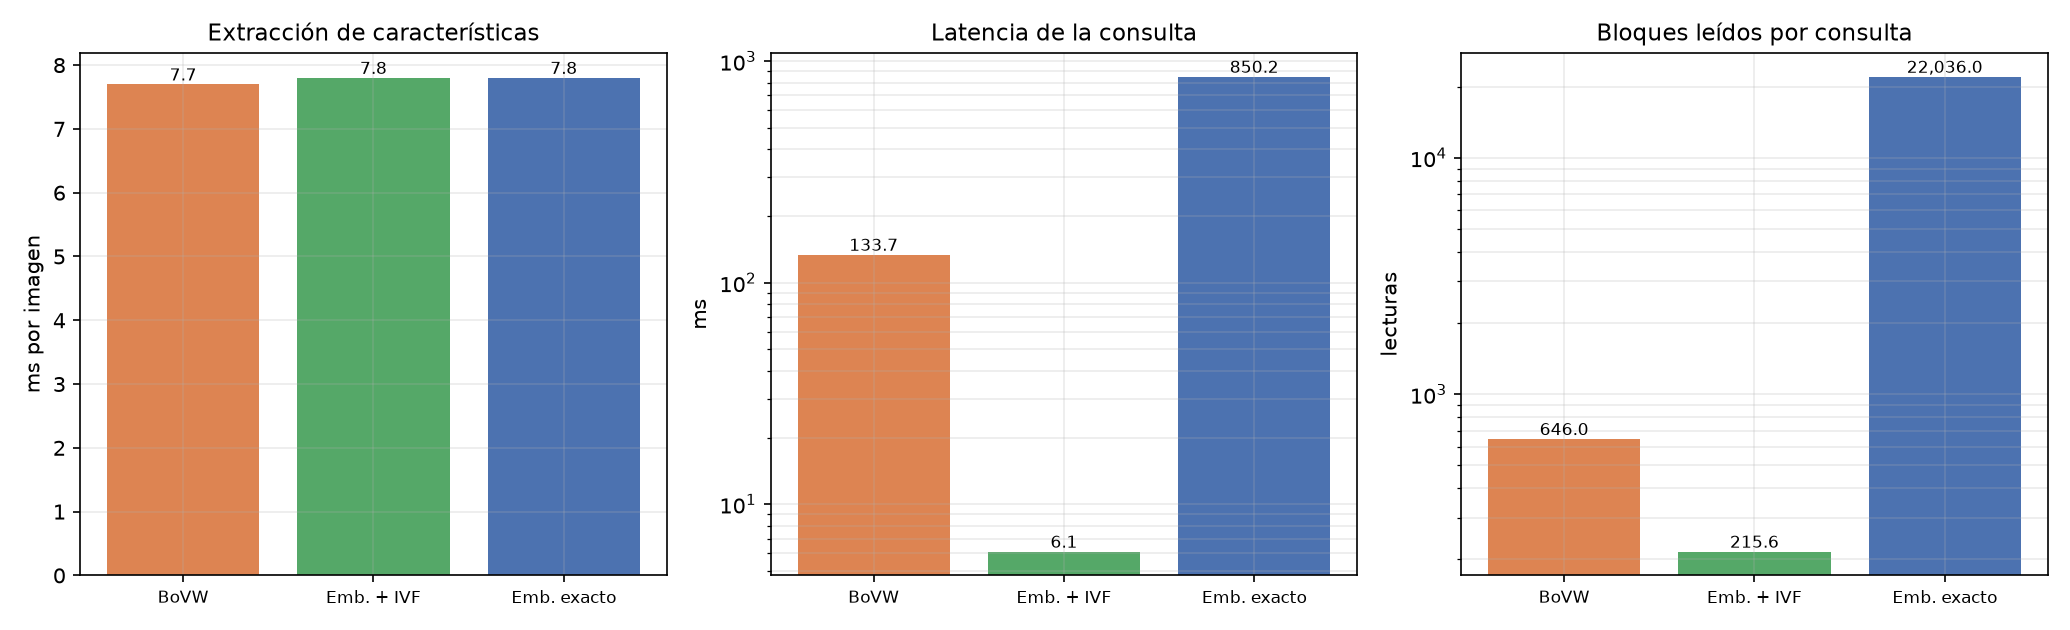
\includegraphics[width=0.92\textwidth]{exp7_cost.png}
\caption{Experimento 7: precisión global y por tipo de artículo (arriba) y costos (abajo).}
\label{fig:exp7}
\end{figure}

\begin{table}[H]
\centering\scriptsize
\resizebox{\ifdim\width>\textwidth\textwidth\else\width\fi}{!}{\begin{tabular}{@{}lrrrrrr@{}}
\toprule
 & \multicolumn{2}{c}{BoVW} & \multicolumn{2}{c}{Embedding + IVF} & \multicolumn{2}{c}{Embedding exacto} \\
Tipo de artículo & P@5 & P@10 & P@5 & P@10 & P@5 & P@10 \\
\midrule
Tshirts & 0.63 & 0.62 & 0.93 & 0.91 & 0.93 & 0.91 \\
Shirts & 0.82 & 0.73 & 0.91 & 0.89 & 0.92 & 0.90 \\
Casual Shoes & 0.52 & 0.49 & 0.81 & 0.78 & 0.82 & 0.79 \\
Watches & 0.76 & 0.77 & 1.00 & 0.99 & 1.00 & 0.99 \\
Sports Shoes & 0.34 & 0.35 & 0.71 & 0.71 & 0.73 & 0.71 \\
Kurtas & 0.61 & 0.53 & 0.62 & 0.59 & 0.64 & 0.60 \\
Tops & 0.30 & 0.20 & 0.47 & 0.38 & 0.46 & 0.36 \\
Handbags & 0.56 & 0.55 & 0.89 & 0.90 & 0.89 & 0.90 \\
Heels & 0.10 & 0.11 & 0.68 & 0.64 & 0.66 & 0.60 \\
Sunglasses & 0.95 & 0.94 & 0.98 & 0.99 & 0.98 & 0.99 \\
Wallets & 0.87 & 0.83 & 0.92 & 0.90 & 0.92 & 0.90 \\
Flip Flops & 0.37 & 0.34 & 0.71 & 0.69 & 0.69 & 0.68 \\
Sandals & 0.20 & 0.21 & 0.63 & 0.58 & 0.62 & 0.58 \\
Briefs & 0.29 & 0.28 & 0.95 & 0.94 & 0.95 & 0.94 \\
Belts & 0.65 & 0.63 & 0.95 & 0.95 & 0.95 & 0.95 \\
\bottomrule
\end{tabular}
}
\caption{Experimento 7: precisión por tipo de artículo.}
\label{tab:exp7tipos}
\end{table}

\paragraph{Análisis.}
\begin{itemize}
\item \textbf{Efectividad}: los \emph{embeddings} alcanzan P@10 = 0.79 frente a 0.51 del BoVW, y
  ganan en los 15 tipos. El BoVW funciona bien cuando la categoría tiene una textura local
  característica (gafas 0.95, billeteras 0.83, relojes 0.77, camisas 0.74) y falla cuando lo que
  distingue a la prenda es la forma global o es parecida a otra categoría: tacones (0.11), sandalias
  (0.21), \emph{tops} (0.20). SIFT describe esquinas y bordes locales, y el histograma descarta la
  disposición espacial; además, en imágenes de $60\times80$ hay pocos puntos de interés (75 en
  promedio). La ResNet-18 codifica forma y contexto global aprendidos en ImageNet. Las dos
  representaciones confunden categorías visualmente cercanas (\emph{tops} con camisetas, sandalias
  con chanclas).
\item \textbf{IVF frente a exacto}: la precisión del índice aproximado con \code{probes} = 5 es
  indistinguible de la del $k$-NN exacto (0.789 y 0.786): los pocos vecinos que el IVF cambia son
  igual de relevantes.
\item \textbf{Extracción}: ambas cuestan $\approx$8\,ms por imagen (SIFT en CPU; ResNet-18 en la GPU
  integrada, 4.2\,ms por imagen en lotes de 256). El BoVW necesita además entrenar el \emph{codebook}
  (37\,s de K-Means para 1\,000 palabras).
\item \textbf{Consulta}: el \emph{embedding} con IVF responde en 6\,ms leyendo 216 bloques; el BoVW
  tarda 134\,ms y lee 646, porque una imagen de consulta tiene $\approx$64 palabras visuales, muchas
  muy frecuentes (un vocabulario de solo 1\,000 palabras repartido en 44\,072 imágenes da listas de
  posteo de miles de entradas), y hay que recorrer la lista de cada una. El $k$-NN exacto lee las
  22\,036 páginas de la tabla (850\,ms).
\end{itemize}

%------------------------------------------------------------------------------------------
\subsection{Experimento 8: eficiencia frente a calidad en la búsqueda aproximada}

200 consultas (vectores del catálogo con ruido gaussiano, renormalizados) sobre los 44\,072
\emph{embeddings} de 128 dimensiones; $k=10$. La verdad base es el $k$-NN lineal exacto. Se varía
\code{ivf.probes} y el número de celdas (\code{lists} $=\sqrt N/4$, $\sqrt N$ y $4\sqrt N$).

\begin{table}[H]
\centering\scriptsize
\resizebox{\ifdim\width>\textwidth\textwidth\else\width\fi}{!}{\begin{tabular}{@{}rrrrrrrr@{}}
\toprule
\code{lists} & \code{probes} & Recall@10 (\%) & ms & lecturas & en el índice & en la tabla & vectores comparados (\%) \\
\midrule
52 & 1 & 80.8 & 2.68 & 161.3 & 151.3 & 10.0 & 2.3 \\
 & 2 & 92.7 & 4.77 & 293.6 & 283.6 & 10.0 & 4.4 \\
 & 5 & 99.2 & 11.32 & 676.3 & 666.3 & 10.0 & 10.4 \\
 & 10 & 99.9 & 21.77 & 1\,296.7 & 1\,286.7 & 10.0 & 20.2 \\
 & 20 & 99.9 & 42.79 & 2\,433.3 & 2\,423.3 & 10.0 & 38.2 \\
 & 50 & 99.9 & 111.70 & 6\,070.5 & 6\,060.5 & 10.0 & 95.8 \\
 & 52 & 100.0 & 112.79 & 6\,336.0 & 6\,326.0 & 10.0 & 100.0 \\
\addlinespace
209 & 1 & 69.4 & 1.08 & 76.5 & 66.5 & 10.0 & 0.6 \\
 & 2 & 84.1 & 1.97 & 112.1 & 102.1 & 10.0 & 1.1 \\
 & 5 & 95.9 & 3.23 & 211.8 & 201.8 & 10.0 & 2.7 \\
 & 10 & 98.6 & 5.79 & 363.0 & 353.0 & 10.0 & 5.1 \\
 & 20 & 99.5 & 11.12 & 667.7 & 657.7 & 10.0 & 9.8 \\
 & 50 & 99.9 & 27.25 & 1\,556.9 & 1\,546.9 & 10.0 & 23.8 \\
 & 100 & 100.0 & 51.47 & 3\,030.7 & 3\,020.7 & 10.0 & 46.8 \\
 & 209 & 99.9 & 111.22 & 6\,425.0 & 6\,415.0 & 10.0 & 100.0 \\
\addlinespace
836 & 1 & 57.7 & 1.30 & 140.7 & 130.7 & 10.0 & 0.2 \\
 & 2 & 73.2 & 1.41 & 151.2 & 141.2 & 10.0 & 0.3 \\
 & 5 & 88.9 & 1.98 & 180.9 & 170.9 & 10.0 & 0.8 \\
 & 10 & 95.5 & 2.85 & 228.8 & 218.8 & 10.0 & 1.5 \\
 & 20 & 98.6 & 4.11 & 315.3 & 305.3 & 10.0 & 2.8 \\
 & 50 & 99.8 & 8.33 & 559.1 & 549.1 & 10.0 & 6.5 \\
 & 100 & 100.0 & 15.16 & 955.4 & 945.4 & 10.0 & 12.4 \\
 & 836 & 99.9 & 116.99 & 6\,786.0 & 6\,776.0 & 10.0 & 100.0 \\
\addlinespace
\multicolumn{2}{@{}l}{$k$-NN exacto (secuencial)} & 100.0 & 878.85 & 22\,036.0 & 0.0 & 22\,036.0 & 100.0 \\
\bottomrule
\end{tabular}
}
\caption{Experimento 8: Recall@10, latencia y bloques leídos (directorio y listas del IVF, más los 10
registros de la tabla).}
\label{tab:exp8}
\end{table}

\begin{figure}[H]
\centering
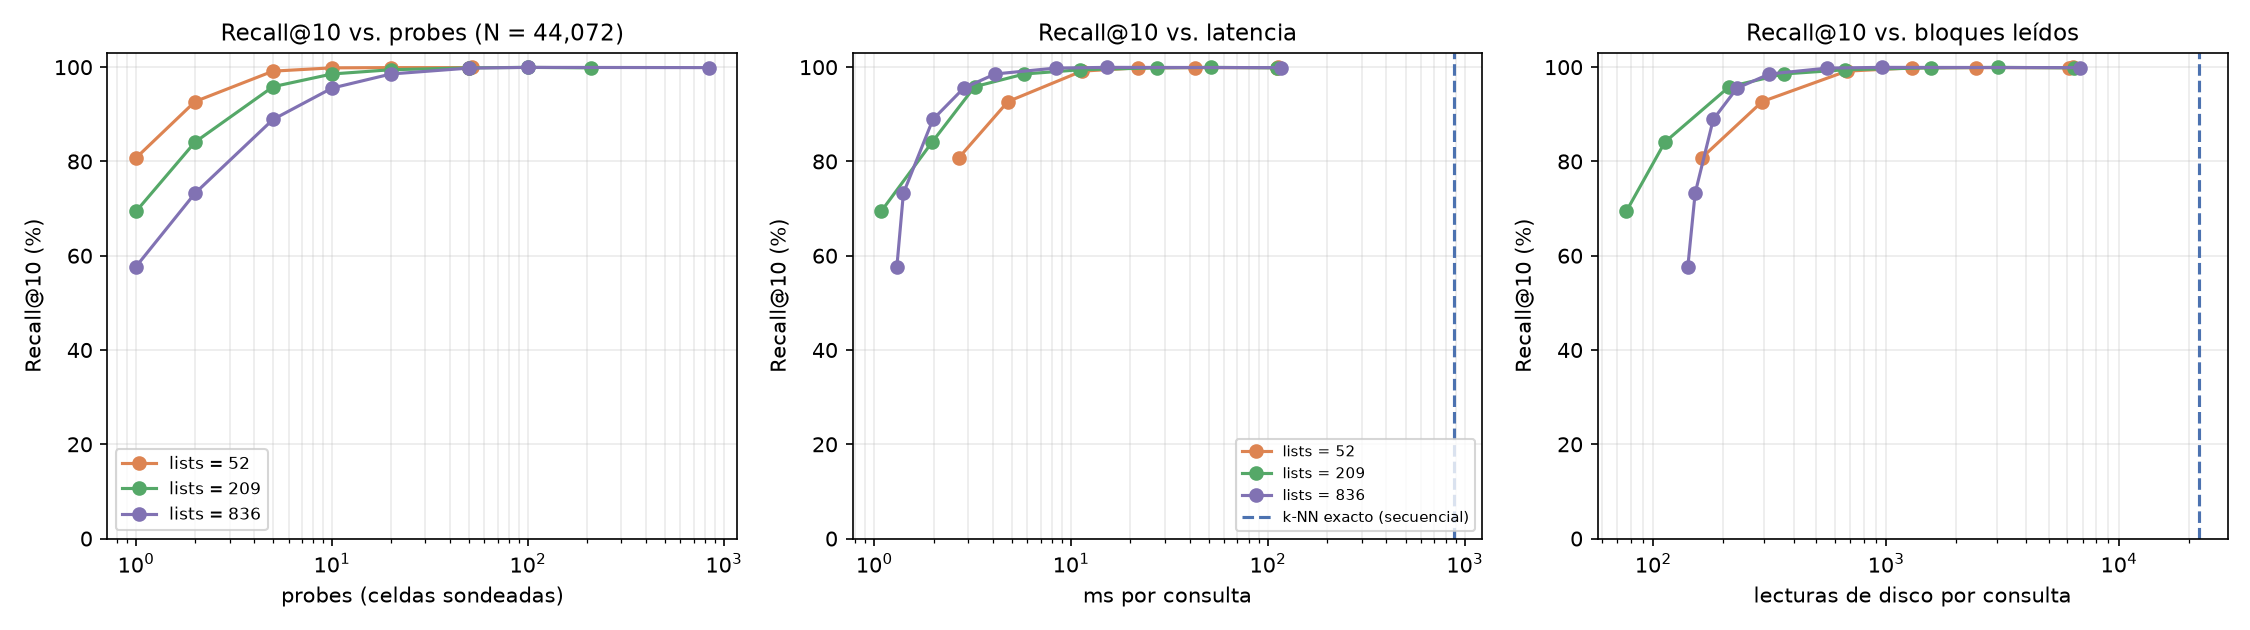
\includegraphics[width=\textwidth]{exp8_recall.png}
\caption{Experimento 8: curvas de compromiso entre Recall@10, \code{probes}, latencia y bloques
leídos. La línea vertical es el $k$-NN exacto por recorrido secuencial.}
\label{fig:exp8}
\end{figure}

\paragraph{Análisis.}
\begin{itemize}
\item \textbf{El compromiso}: con $C=\sqrt N=209$ celdas, \code{probes} = 1 compara solo el 0.6\,\%
  de los vectores y ya encuentra el 69\,\% de los vecinos verdaderos; con \code{probes} = 5 el
  recall es 95.9\,\% (212 bloques, 3.2\,ms) y con \code{probes} = 10, 98.6\,\% (363 bloques,
  5.8\,ms). El $k$-NN exacto lee 22\,036 bloques y tarda 879\,ms: el IVF con \code{probes} = 10 lee
  el \textbf{1.6\,\%} de los bloques y es \textbf{150 veces más rápido} a cambio de perder 1.4 puntos
  de recall. El recall crece de forma cóncava: cada celda adicional aporta menos vecinos nuevos.
\item \textbf{El costo sigue la fórmula}: las lecturas son las páginas del directorio
  ($\lceil C/7\rceil$ = 30 con $C=209$) más las de las celdas sondeadas ($\approx$\,probes\,$\cdot
  N/(7C)$ = 30 por celda) más los 10 registros: con \code{probes} = 5, $30+151+10\approx$ 191
  estimadas y 212 medidas (las celdas cercanas a la consulta son más densas que el promedio).
\item \textbf{Número de celdas}: con pocas celdas ($C=52$) cada una es grande: \code{probes} = 1 ya
  da 80.8\,\% de recall, pero leyendo 161 bloques. Con muchas ($C=836$) las celdas son pequeñas y se
  alcanza el mismo recall comparando menos vectores (98.6\,\% con el 2.8\,\% de los vectores, frente
  al 5.1\,\% con $C=209$), pero el directorio crece (120 páginas que se leen en cada consulta) y
  domina cuando \code{probes} es pequeño. En bloques leídos para un recall de $\approx$98.6\,\%:
  315 con $C=836$ frente a 363 con $C=209$; con $C=52$ hacen falta 676 para llegar al 99.2\,\%. $C=\sqrt N$ es un buen punto
  medio; con más celdas convendría mantener los centroides en memoria.
\item \textbf{Exactitud en el límite}: con \code{probes} $=C$ se comparan todos los vectores; el
  recall medido es 99.9\,\% y no 100\,\% porque el catálogo tiene imágenes duplicadas con el mismo
  \emph{embedding} y los empates en la posición 10 se resuelven distinto que en la verdad base.
  Incluso así el IVF exhaustivo lee 6\,425 bloques frente a 22\,036, porque sus páginas solo guardan
  $\langle\text{RID}, \vec v\rangle$ (7 por página) y la tabla guarda registros de 1\,708 bytes (2 por
  página).
\end{itemize}
